\chapter{Определение аномалий} \label{ch:ch2}

\section{Основы алгоритмов} \label{sec:ch2/sec1}

Задачу поиска аномалий можно отнести к классу задач обучения без учителя. Суть поиска аномалий заключается в том, чтобы найти в выборке объекты, которые не похожи на большинство объектов выборки, то есть те, которые выделяются на фоне других.

Часто бывает так, что аномальных объектов либо нет вообще, либо их очень мало и неизвестно где именно в выборке они находятся. Поэтому обычно поиск аномалий относится к классу задач обучения без учителя (так как отсутствуют размеченные данные).

\subsection{Анализ}

В качестве источника информации используются статьи \cite{dai, hodge, vakili, varun, billor, wilkinson}. Помимо статей интерес представляют наборы данных, которые тоже предстояло найти. Среди наборов данных есть хорошо известный MNIST с набором изображений рукописных цифр, а также данные касательно разных типах стёкол, о заболеваниях сердца, о свободных электронах в ионосфере Земли и другие.

В этой работе рассматриваются стационарные данные. Поиск аномалий во временных рядах и прогнозирование временных рядов находятся за рамками рассматриваемой в работе темы.

\subsection{Результат работы алгоритмов}

Результатом работы алгоритма для поиска аномалий могут быть как \textbf{степени аномалии} (anomaly scores), так и \textbf{бинарные метки} (binary labels).

В случае, когда алгоритм выдаёт \textbf{степень аномалии}, под степенью понимается уровень вероятности того, что объект является аномалией.

В случае \textbf{бинарных меток} алгоритм сразу указывает на нормальные (обычно обозначаемые как $0$) и аномальные (обозначаемые как $1$) данные. Несмотря на то, что некоторые алгоритмы детектирования аномалий возвращают бинарные метки напрямую, степени аномалий тоже могут быть переведены в бинарное представление. $0$ или $1$ содержат меньше информации, чем степень аномалии. Тем не менее, это конечный результат, по которому обычно принимается решение об аномальности объекта выборки.

\clearpage

\section{Классификация методов определения аномалий} \label{sec:ch2/sec2}

Большинство методов определения аномалий используют метки, по которым можно определить, является ли объект выборки нормальным или аномальным. Поиск или сбор размеченных данных, которые будут точными и хорошо описывать рассматриваемую проблему, чтобы хорошо обучить алгоритмы, довольно сложно и дорого.

\noindent Обычно выделяют три типа методов поиска аномалий:

\begin{enumerate}
	\item \textbf{Supervised методы (обучение с учителем)}

Предполагается, что имеется доступ к обучающим данным с точными и репрезентативными метками для нормальных и аномальных объектов. В таком случае обычно разрабатывают предсказательную модель для обоих классов. После обучения на тренировочных данных к каждому объекту из тестовой выборки применяется алгоритм, чтобы определить класс объекта. Проблема такого подхода заключается в том, что получить точные и репрезентативные метки, особенно для аномалий, сложно. Такая ситуация довольно распространена в таких областях, как обнаружение мошенников в банковском секторе (сложно отличить мошенника от обычного пользователя только по действиям).
	
	\item \textbf{Semi-supervised методы (обучение с частичным привлечение учителя)}

Предполагается, что имеются размеченные данные только для нормального класса. Так как для обучения таких алгоритмов не требуются размеченные аномальные данные, они имеют более широкое применение, чем supervised методы.
	\item \textbf{Unsupervised методы (обучение без учителя)}

Такие методы не требуют обучающих данных и поэтому наиболее широко используются. Unsupervised методы поиска аномалий могут нормальные данные из всех представленных и рассматривать отклонение от них как аномалию.
\end{enumerate}
Многие semi-supervised методы могут быть использованы для unsupervised случая. Например, с их помощью можно дополнительно семплировать объекты из выборки, если данных для обучения алгоритма попросту недостаточно.

\subsection{Метрика качества модели}

В качестве основной метрики используется ROC-AUC, что расшифровывается как "receiver operating characteristic -- area under curve" и переводится как "рабочая характеристика приёмника -- площадь под кривой". ROC-кривая позволяет оценить качество бинарной классификации\footnote{бинарная означает, что есть лишь два класса объектов -- например, нормальные и аномальные}. Она показывает соотношение между долей объектов, которые были верно классифицированы как принадлежащие определённому классу (True Positive Rate, TPR), и долей объектов от общего количества объектов, которые этому классу не принадлежат, ошибочно классифицированных как принадлежащие этому классу (False Positive Rate, FPR).

Количественную интерпретацию ROC даёт показатель AUC -- площадь, ограниченная ROC-кривой и осью доли ложных положительных классификаций (False Positive Rate). Чем выше показатель AUC, тем качественнее классификатор, при этом значение $0.5$ демонстрирует непригодность выбранного метода классификации, что эквивалентно случайному выбору. Максимальное значение AUC составляет $1.0$.

\begin{figure}[ht]
  \centering
  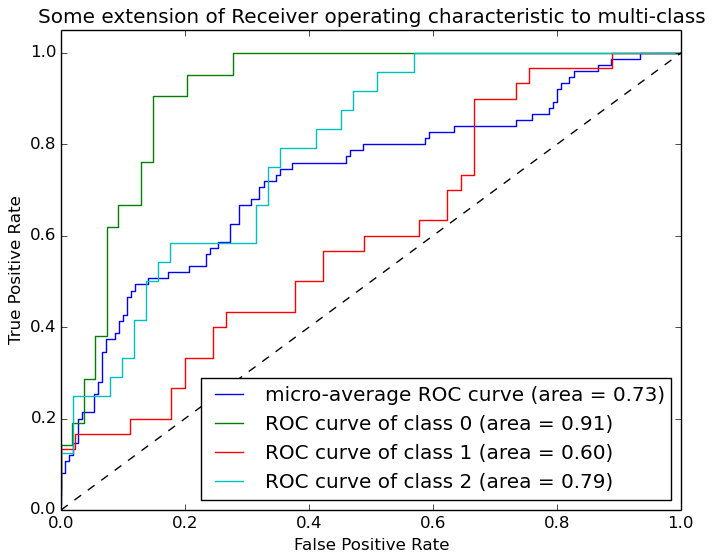
\includegraphics [scale=0.7] {roc_curve}
  \caption{Пример ROC-кривой.}
  \label{fig:roc_curve}
\end{figure}

График на рисунке \ref{fig:roc_curve} был построен с помощью библиотеки scikit-learn\footnote{\url{https://scikit-learn.org/0.15/auto_examples/plot_roc.html}}.

\clearpage

\section{Подходы к решению} \label{sec:ch2/sec3}

Одним из возможных способов определения аномалий является измерение схожести между объектов. У такого способа есть два варианта:
\begin{enumerate}
  \item Восстановление плотности
  \item Классификация
\end{enumerate}

В случае с восстановлением плотности необходимо построить распределение, которое хорошо описывает выборку. И это распределение позволяет посчитать вероятность для нового объекта получить его из распределения, описывающего выборку.

В терминах этого метода аномалия - объект, полученный из другого распределения, описывающего другую выборку данных.

\noindent Есть три подхода:
\begin{enumerate}
  \item Параметрический
  \item Непараметрический
  \item Восстановление смесей
\end{enumerate}

\subsection{Параметрический подход}

Распределение представляется в виде $p(x)=\phi(x\vert\theta)$, где $\theta$ выступает в качестве параметра распределения. Например, в семейство параметрических распределений входит распределение Гаусса -- $\theta=(\mu, \Sigma)$, где $\mu$ -- вектор средних и $\Sigma$ -- ковариационная матрица.

Параметры модели подбираются таким образом, чтобы вероятность объектов из обучающей выборки была максимальной. Для этого обычно пользуются Методом Максимального Правдоподобия (Maximum Likelihood Estimation, MLE):

\[ \sum_{i}\log\phi(x_{i}\vert\theta) \rightarrow \max_{\theta}.\]

В случае нормального распределения формулы для параметров распределения будут иметь следующий вид:

\[\mu = \frac{1}{N}\sum_i x_i,\]

\[\Sigma = \frac{1}{N}\sum_i \left(x_i - \mu\right)\left(x_i - \mu\right)^T.\]

\noindent Тогда алгоритм для определения аномалий будет выглядеть так:
\begin{enumerate}
  \item Получаем новый объект $x$ из выборки
  \item Если $p(x) < t$, то полагаем, что объект $x$ является аномалией
  \item Порог принятия решения $t$ выбирается из априорных соображений
\end{enumerate}

\subsection{Непараметрический подход}

Для восстановления вида распределения вероятности по данным используется формула оценки Парзена-Розенблатта:

\[p_h(x)=\frac{1}{lh}\sum_{i=1}^l K\left(\frac{x-x_i}{h}\right),\]

где $h$ -- ширина окна, $K$ -- ядровая функция (Kernel Function). Функция ядра $K$ должна удовлетворять таким требованиям, как $K(x)=K(-x) \forall x$ и $\int_{-\infty}^{+\infty}K(x)dx=1$.

\begin{figure}[ht]
  \centering
  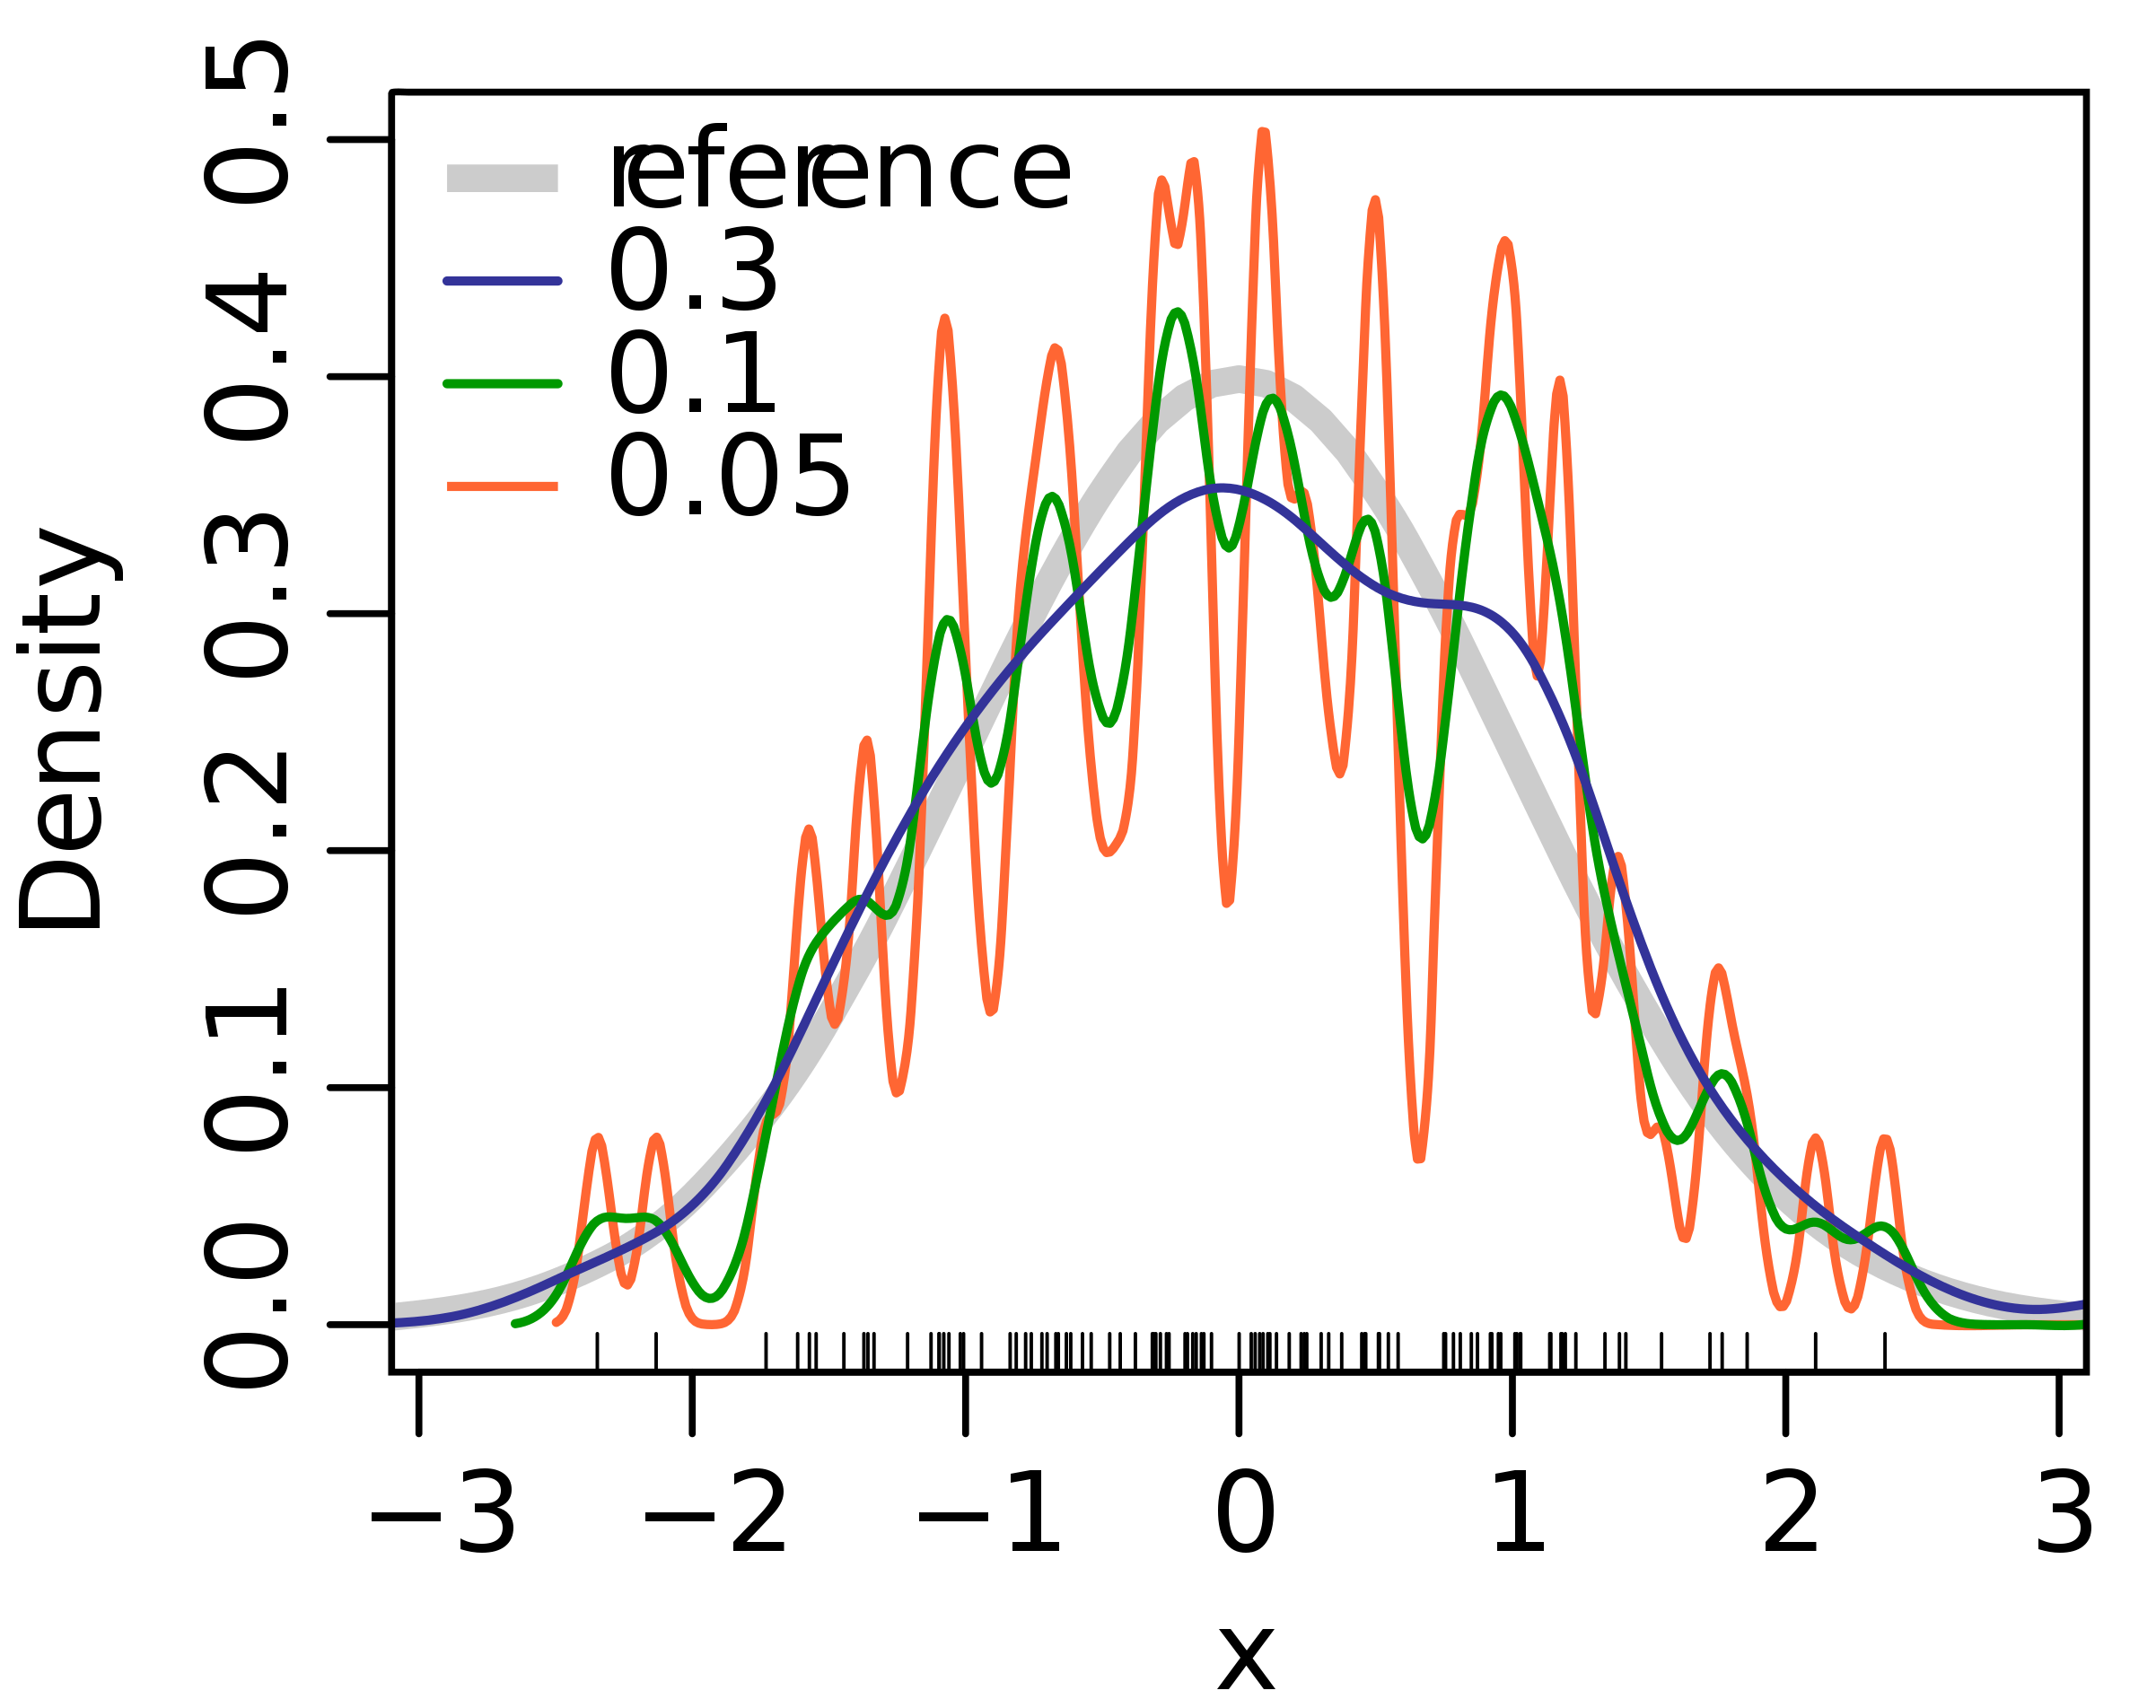
\includegraphics [scale=0.10] {kernel}
  \caption{Ядерная оценка плотности 100 нормально распределённых случайных чисел с использованием различных сглаживающие окон.}
  \label{fig:kernel}
\end{figure}

\noindent Примеры ядерных функций:
\begin{enumerate}
  \item Равномерное: $K(u)=\frac{1}{2}$, $|u|\leq 1$
  \item Треугольное: $K(u)=(1-|u|)$, $|u|\leq 1$
  \item Гауссово: $K(u)=\frac{1}{\sqrt{2\pi}}e^{-\frac{1}{2}u^2}$
\end{enumerate}

\noindent Хорошо обобщается на многомерный случай:

\[p_h(x)=\frac{1}{lV(h)}\sum_{i=1}^l K\left(\frac{\rho(x,x_i)}{h}\right),\]

где $\rho$ -- заданная метрика (например, евклидово расстояние), $V(h)=\int K\left(\frac{\rho(x,x_i)}{h}\right)dx$. Чем выше размерность, тем больше объектов необходимо для лучшей точности алгоритма.

\subsection{Восстановление смесей}

В некоторых случаях параметрического подхода оказывается недостаточно. Например, распределение на~рисунке~\ref{fig:mixture} получено путём семплирования из трёх гауссовых распределений с равными стандартными отклонениями, но разными центрами. Такую выборку можно описать моделью смеси распределений. Для восстановления такой плотности отлично подходит EM-алгоритм.

Введём некоторые обозначения:

\[p(x)=\sum_{j=1}^K w_j p_j(x)\]

-- смесь распределений (взвешенная сумма), где $p_j(x)$ -- компоненты смеси (обычно являющиеся параметрическими распределениями $p_j(x)=\phi(x|\theta_j)$),

\[g_{ji}=p(j|x_i)=\frac{w_jp_j(x_i)}{p(x_i)}\]

-- апостериорная вероятность того, что объект под номером $i$ принадлежит компоненте смеси под номером $j$.

\noindent Тогда EM-алгоритм будет выглядеть следующим образом:
\begin{enumerate}
  \item На E-шаге рассчитывается апостериорная вероятность $g_{ji}$
  \item На M-шаге рассчитываются новые веса $w_j=\frac{1}{N}\sum_{i=1}^N g_{ji}$ и обновляется оценка на параметры $\theta$: $\theta_j = \arg\max_{\theta} \sum_{i=1}^N g_{ji} \log\phi(\theta|x)$
\end{enumerate}


\begin{figure}[ht]
  \centering
  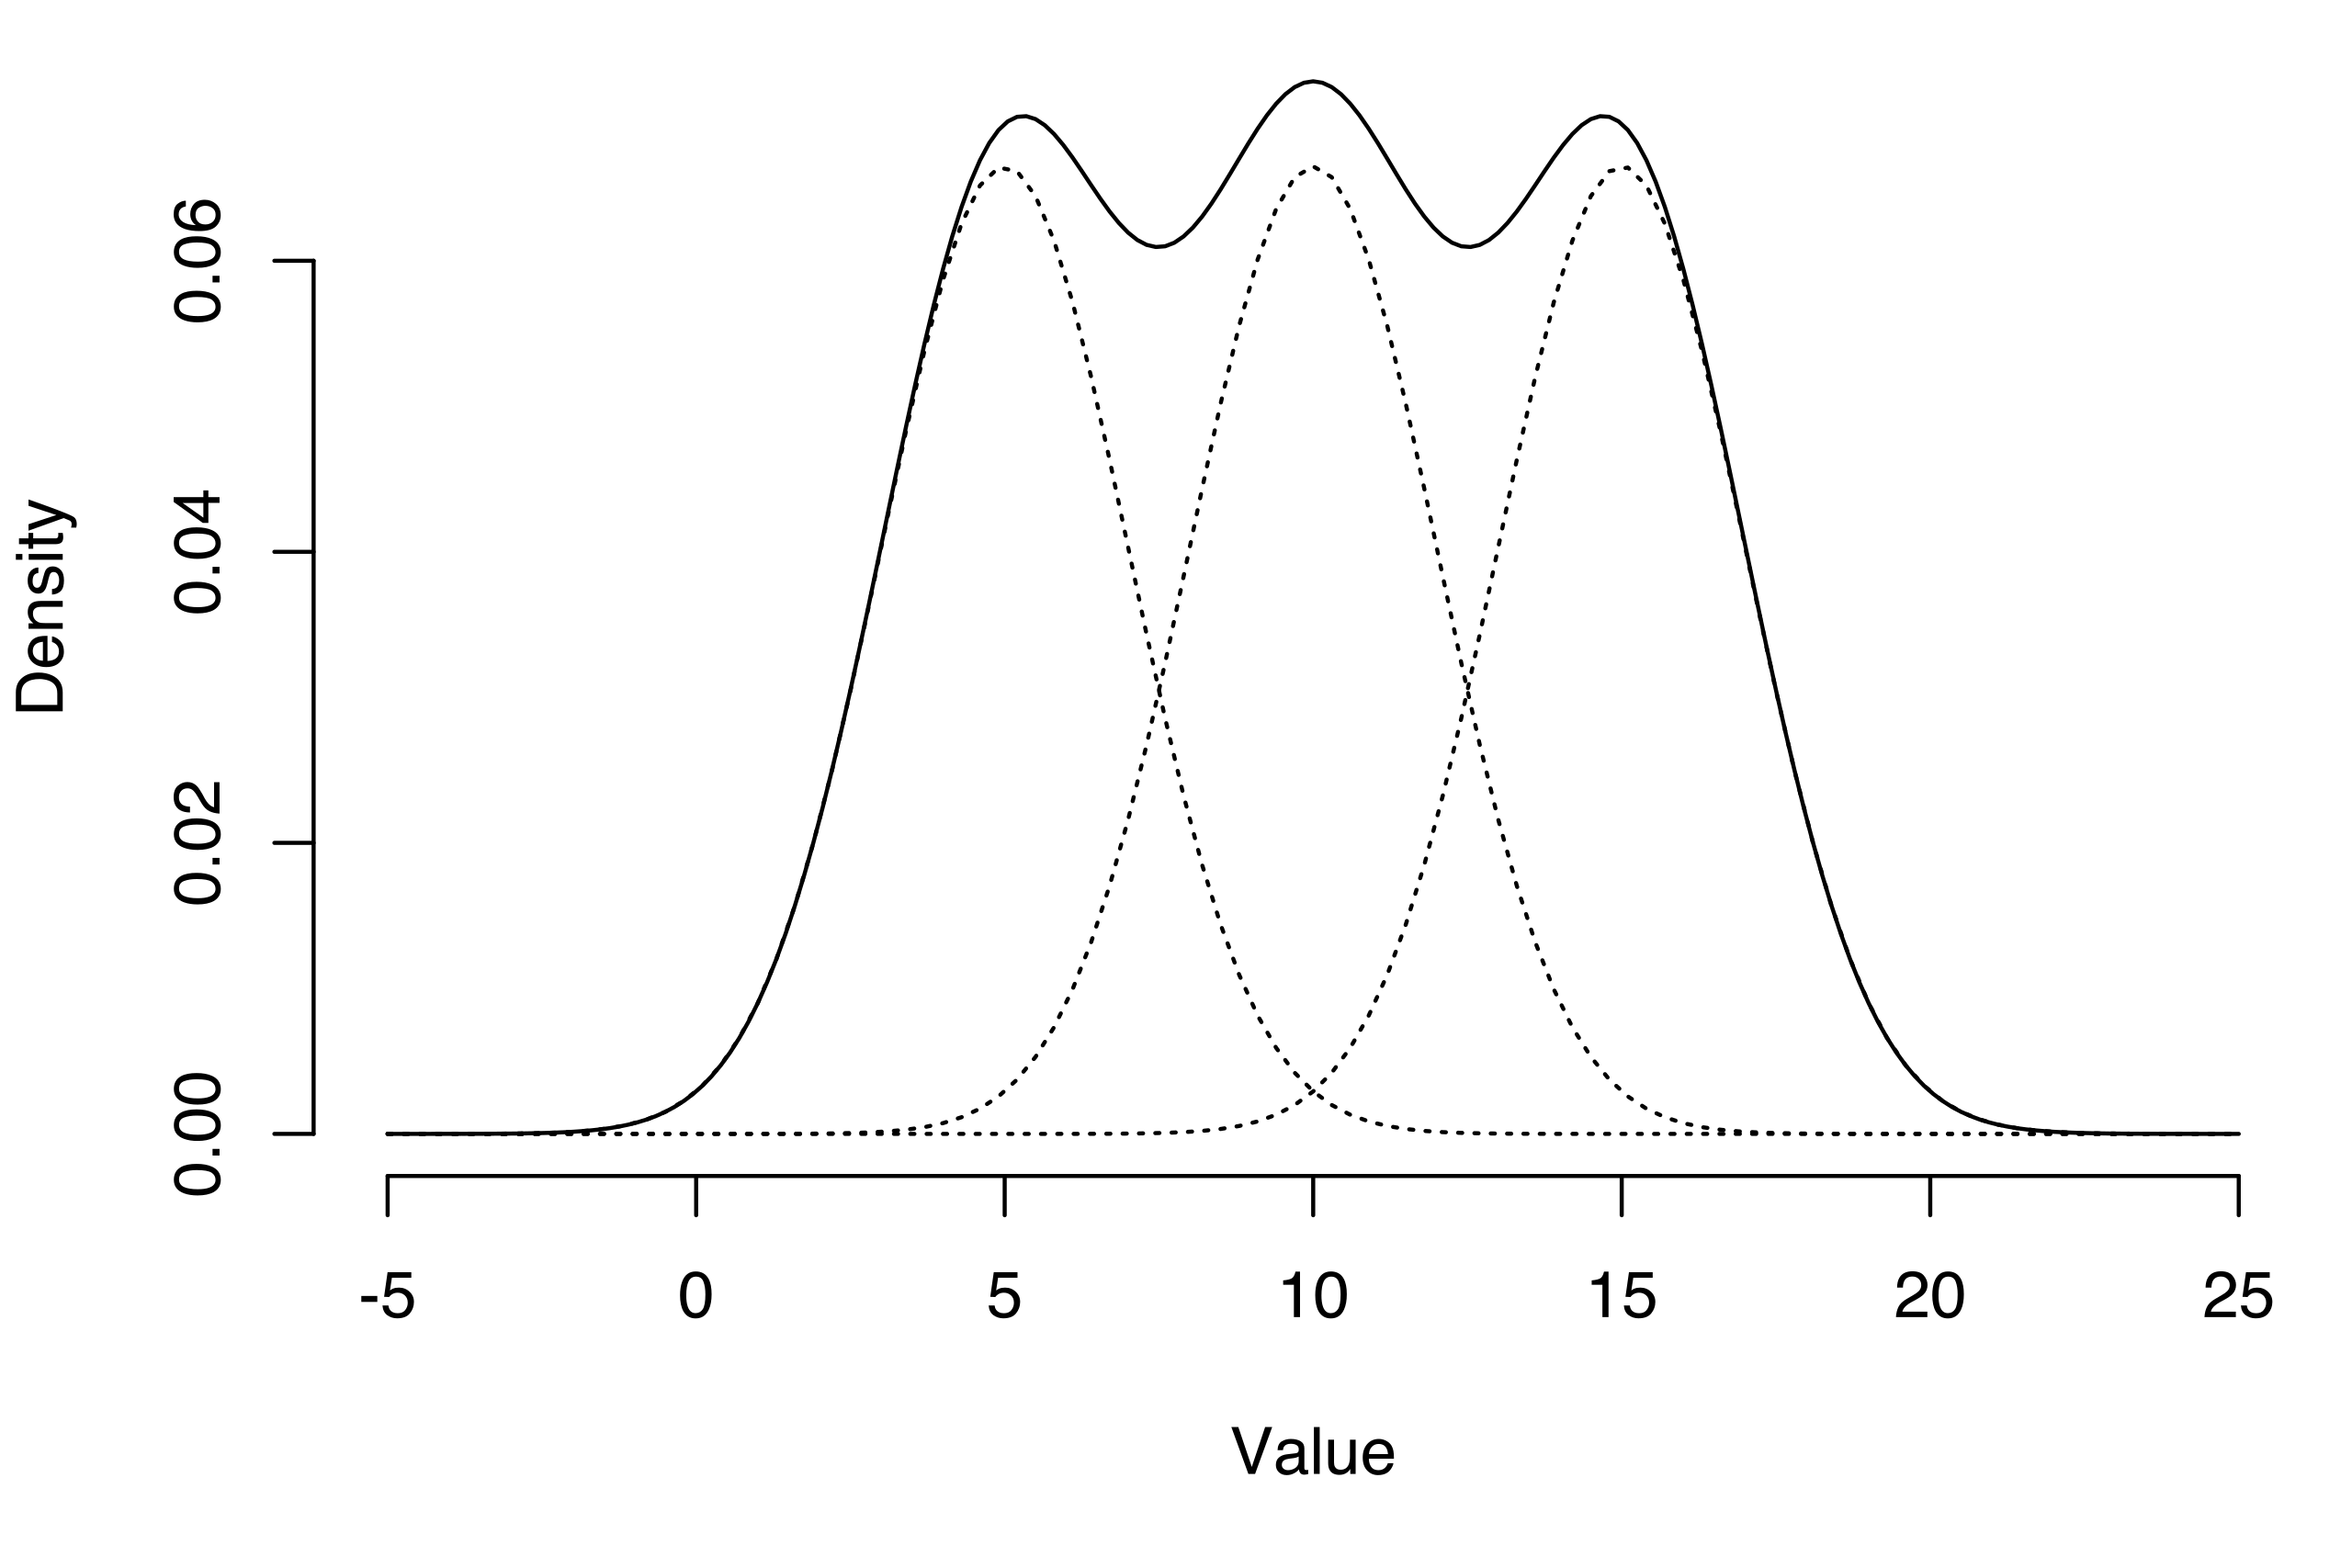
\includegraphics [scale=0.15] {mixture}
  \caption{Плотность распределения смеси, состоящей из трёх нормальных распределений ($\mu = [5, 10, 15]$, $\sigma = 2$) с одинаковыми весами.}
  \label{fig:mixture}
\end{figure}

\noindent Существуют ещё Автокодировщики, которые хорошо справляются с понижением размерности многомерных данных и с помощью которых можно хорошо семплировать из заданного распределения \cite{karazeev}. Но такой подход лежит за рамками этой бакалаврской работы.

\clearpage

%\begin{figure}[ht]
%  \centering
%  
\includegraphics [scale=0.27] {latex}
%  \caption{TeX.}
%  \label{fig:latex}
%\end{figure}
